\documentclass[a4paper,12pt]{article}

% Author information
\author{Eugen-Cristian RAVARIU, Vladislav TIFTILOV}

% Package imports
\usepackage[utf8]{inputenc}
\usepackage[margin=2cm]{geometry}
\usepackage{amsmath}
\usepackage{amsfonts}
\usepackage{amssymb}
\usepackage{graphicx}
\usepackage{float}
\usepackage{caption}
\usepackage{setspace}
\usepackage{hyperref}
\usepackage{cite} % For bibliography

% Times New Roman font
\usepackage[T1]{fontenc}    % Use T1 font encoding
\usepackage{lmodern}        % Latin Modern typefaces, including typewriter
\usepackage{mathptmx}

% Title and subtitle formatting
\usepackage{titlesec}

% Line spacing
\setstretch{1.15}

% Figure, table, and algorithm numbering
\renewcommand{\thefigure}{\arabic{figure}}
\renewcommand{\thetable}{\arabic{table}}

% Document starts
\begin{document}

% Title Section
\begin{titlepage}
    \centering
    National University of Science and Technology Politehnica Bucharest\\
    \vfill
    {\bfseries\fontsize{14pt}{14pt} DataDot}\par
    \vspace{0.5cm}
    {\bfseries\fontsize{12pt}{12pt} End-to-End Data Pipeline}\par
    \vspace{2.5cm}
    Eugen-Cristian RAVARIU, Vladislav TIFTILOV\\
    \vfill
    \date{\today}
\end{titlepage}

% Abstract Section
\section{Abstract}
\label{sec:abstract}

Fast growth across all domains of our daily life has determined the need for storing and processing 
large amounts of data. The challenges a developer faces are not only caused by the amount of data, 
but also by its variety and quality. Sometimes, the most challenging part is to semantically understand 
the data and to extract valuable information from it.

This paper presents an end-to-end data pipeline that aims to automate the process of data transformation 
and visualization. During the project, we discovered the importance of data quality, which led us to change 
the dataset several times in order to get the most meaningful insights. To face real challenges of the 
big data world, we purposely chose a dataset that is both large and complex. The dataset contains 
information about movies, including the title, genre, rating, runtime, and the number of votes.

We started by cleaning the data and aggregating the information, then we performed statistical 
analysis to generate insights. The decision to use Azure was made because we wanted our solution 
to be end-to-end—from data ingestion to visualization—on a single cloud platform. Another reason 
was the need for scalability, as the dataset contains over 8GB of data, and Azure provides the 
necessary resources to handle large amounts of data. The data pipeline was implemented using 
Azure Data Factory, Azure Databricks, Azure Synapse Analytics, and Power BI.

The decision to go with a movies dataset was made because we wanted to analyze trends in 
the movie industry, but also due to the complexity of the dataset, which allowed us to gain 
insights across multiple dimensions, such as genre, rating, runtime, and region.

\newpage
\tableofcontents  % Generates the Table of Contents
\newpage

% Main Content
\section{Introduction}
\label{sec:introduction}

Movies are a popular form of entertainment and are watched by millions of people around the world. 
The dataset contains information about movies, including the title, genre, rating, runtime, and the 
number of votes. The goal of this project is to analyze the dataset and provide insights into the 
distribution of movies based on the genre, rating, runtime, and region. The analysis will help us 
understand the trends in the movie industry and identify the most popular genres, regions, and runtime. 
The insights will be visualized using Power BI to create a dashboard that can be used to explore the 
data and gain a deeper understanding of the movie industry.

The main challenges of the project is caused by the size of the dataset and the need to automate 
the data transformation process. The dataset contains over 8GB of data and is stored in multiple 
CSV files. The data transformation process involves cleaning the data, aggregating the information, 
and performing statistical analysis to generate insights. The data pipeline will be implemented using 
Azure Data Factory, Azure Databricks, Azure Synapse Analytics, and Power BI to automate the data 
transformation process and create a dashboard for visualization.

\section{Opinion}
\label{sec:opinion}

In this section we will present our opinions on the project, the challenges we faced, and the lessons we learned.

\subsection{Eugen-Cristian RAVARIU}

TBA

\subsection{Vladislav TIFTILOV}



\section{Implementation}
\label{sec:implementation}

The end-to-end data pipeline was implemented using Azure Data Factory, Azure Databricks, Azure Synapse Analytics, and Power BI. The pipeline consists of the following stages: data ingestion, data preprocessing, data integration, and data visualization. The implementation steps are described below.

\subsection{Dataset Used: IMDb Dataset}

The IMDb dataset contains information about the film industry and consists of five tables:
\begin{enumerate}
    \item \textbf{name\_basics}: Includes information about individuals, such as names, birth and death dates, occupations, and associated movies.
    \item \textbf{title\_basics}: Contains details about movies, such as type, title, release year, duration, and genres.
    \item \textbf{title\_akas}: Offers alternative titles and translations of the title in other languages.
    \item \textbf{title\_principals}: Specifies the roles of each person involved in creating the movie, including details about actors' roles.
    \item \textbf{title\_ratings}: Comprises IMDb movie scores and the number of reviews.
\end{enumerate}

Link to the dataset: \href{https://www.kaggle.com/datasets/ashirwadsangwan/imdb-dataset/data}{IMDb Dataset}

\section{Data Ingestion Implementation Steps}

\subsection{Creating a Data Lake}
The first step involved building a data lake, a storage infrastructure designed for managing large volumes of data. Two containers were created:
\begin{itemize}
    \item \textbf{bronze}: Used for storing raw, unmodified data.
    \item \textbf{silver}: Used for storing preprocessed data.
\end{itemize}

\subsection{Configuring Access to the Data Lake}
Using a dedicated notebook, \texttt{mountStorage.ipynb}, the containers were mounted in 
Azure Databricks, a scalable data processing platform. This configuration enabled direct 
access to files stored in the data lake from notebooks.

\subsection{Downloading and Storing Raw Data}
The dataset download process was implemented in the notebook \texttt{imdb2bronze.ipynb}. The data 
was obtained from the Kaggle platform using the official library in a Jupyter Notebook environment 
within Azure Databricks. The data, available as TSV (Tab Separated Values) files, was read using 
Apache Spark and stored in the \textbf{bronze} container in Parquet format.

\subsection{Data Preprocessing}
Data preprocessing is a critical step in preparing data for analysis. This process was implemented in the notebook \texttt{bronze2silver.ipynb}, including the following steps:

\begin{itemize}
    \item \textbf{Column name transformation}: Conversion of column names to \texttt{snake\_case}.
    \item \textbf{Null value replacement}: The string \texttt{\textbackslash N}, used in the original dataset for missing values, was replaced with \texttt{NULL}.
    \item \textbf{Data type conversion}: Columns containing numbers stored as strings were converted to appropriate numeric types (e.g., \texttt{int} or \texttt{decimal}).
    \item \textbf{Redundancy elimination}: Columns that did not add value to the analysis were removed.
    \item \textbf{Data normalization}: Columns containing lists of values were split into new tables, improving the structure and integrity of the data.
\end{itemize}

The preprocessed data was saved in the \textbf{silver} container in Delta format.

\subsection{Creating SQL Views in Azure Synapse}
For each table in the \textbf{silver} container, views were created in Azure Synapse Analytics. This step facilitated data access and integration in subsequent project stages.

\section{Conclusions}
\label{sec:conclusions}

As a result of the project, we were able to extract following insights from the IMDb dataset:

\begin{table}[ht]
    \centering
    \begin{tabular}{|l|p{10cm}|}
    \hline
    \textbf{Analysis Aspect} & \textbf{Details} \\
    \hline
    \textbf{Best rated genres} & History, Documentary, Biography, Animation \\
    \hline
    \textbf{Distribution of movies (year)} & Peak in 2021 (501k movies) \\
    \hline
    \textbf{Most popular genres} & Drama, Comedy, Talk-Show \\
    \hline
    \textbf{Rating distribution} & Gaussian distribution with mean \(\sim 7.4\) \\
    \hline
    \textbf{Runtime average by genre} & Film-Noir (82 mins), Adult (79 mins), Sport (63 mins) \\
    \hline
    \textbf{Average rating by runtime} & Peak at 40 mins (7.41), dips to \(\sim 6\) at 85 mins, then gradually rises to \(\sim 7.45\) at 285 mins \\
    \hline
    \textbf{Distribution by runtime} & Peaks at 20 mins (450k movies), 30 mins (374k), 60 mins (273k) \\
    \hline
    \textbf{Average votes by runtime} & Bell-shaped curve centered \(\sim 90\)–200 mins, peak at 170 mins (13k votes) \\
    \hline
    \textbf{Count of movies by region} & US (946k), GB (118k), IN (334k), CA (194k), FR (185k) \\
    \hline
    \end{tabular}
    \caption{Concatenated Table of Analysis Aspects}
    \label{tab:analysis_aspects}
\end{table}
    
Following are some captures of the Power BI dashboard created for the IMDb dataset:

\begin{figure}[H]
    \centering
    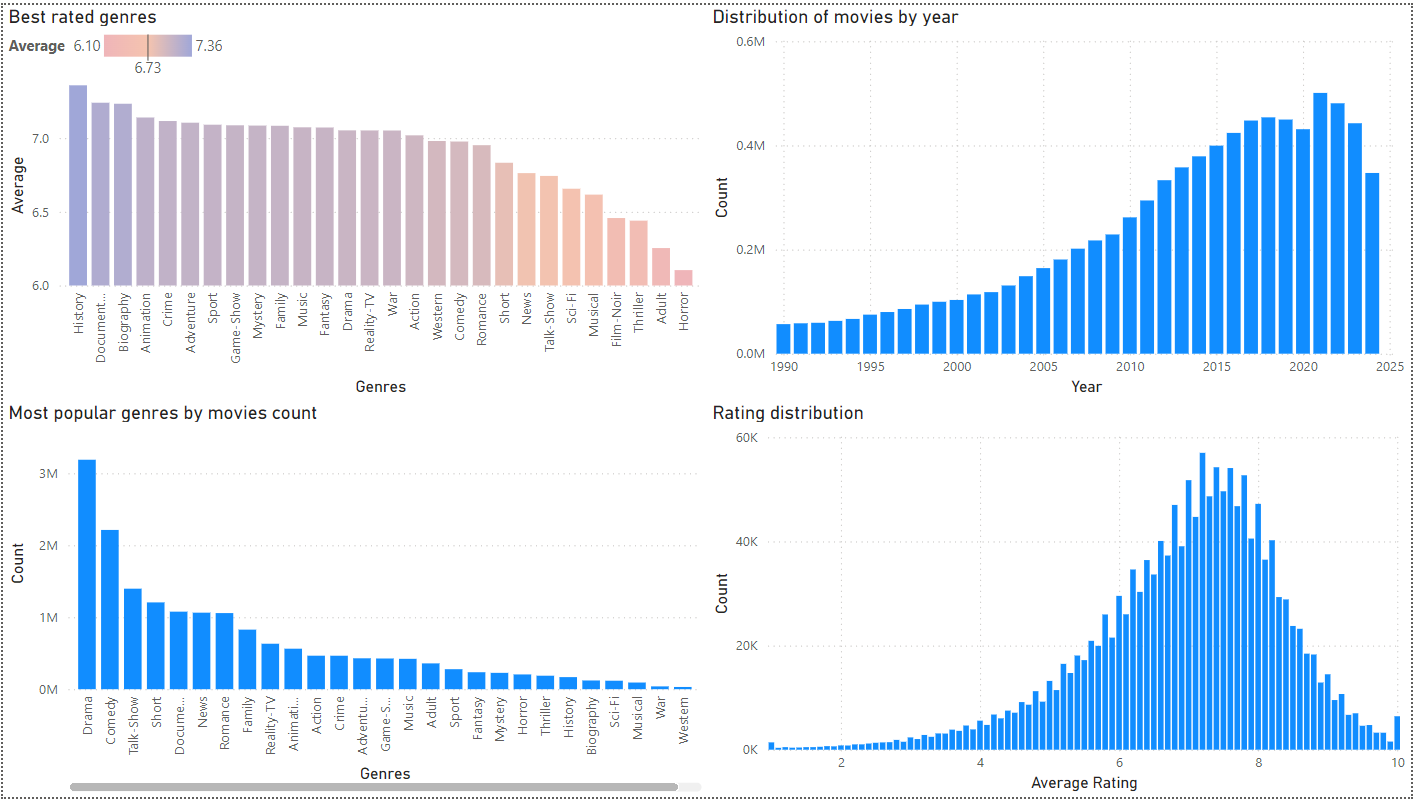
\includegraphics[width=0.8\textwidth]{../assets/movies_summary.png}
    \caption{Summary of Movies Analysis}
    \label{fig:movies_summary}
\end{figure}

\begin{figure}[H]
    \centering
    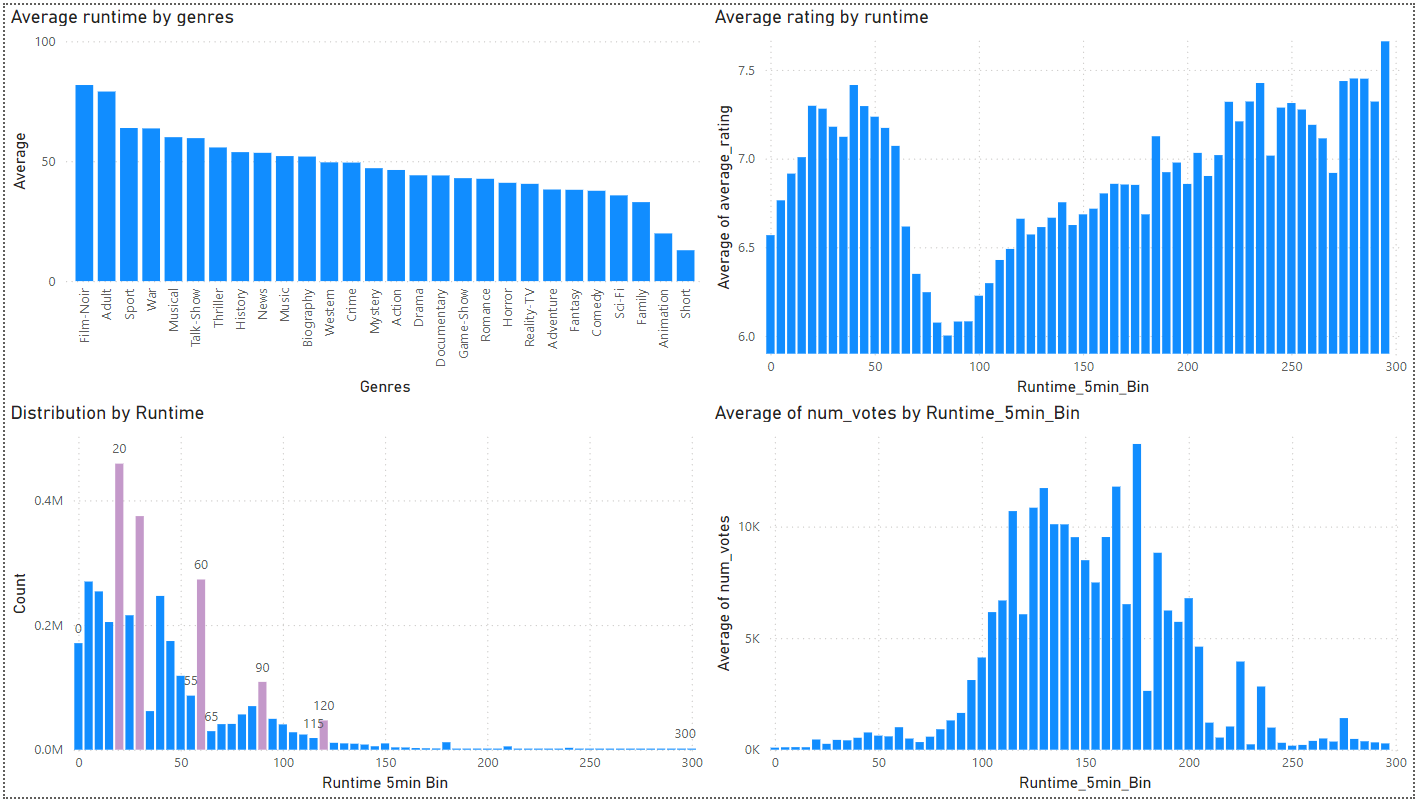
\includegraphics[width=0.8\textwidth]{../assets/movies_runtime.png}
    \caption{Runtime Analysis of Movies}
    \label{fig:movies_runtime}
\end{figure}

\begin{figure}[H]
    \centering
    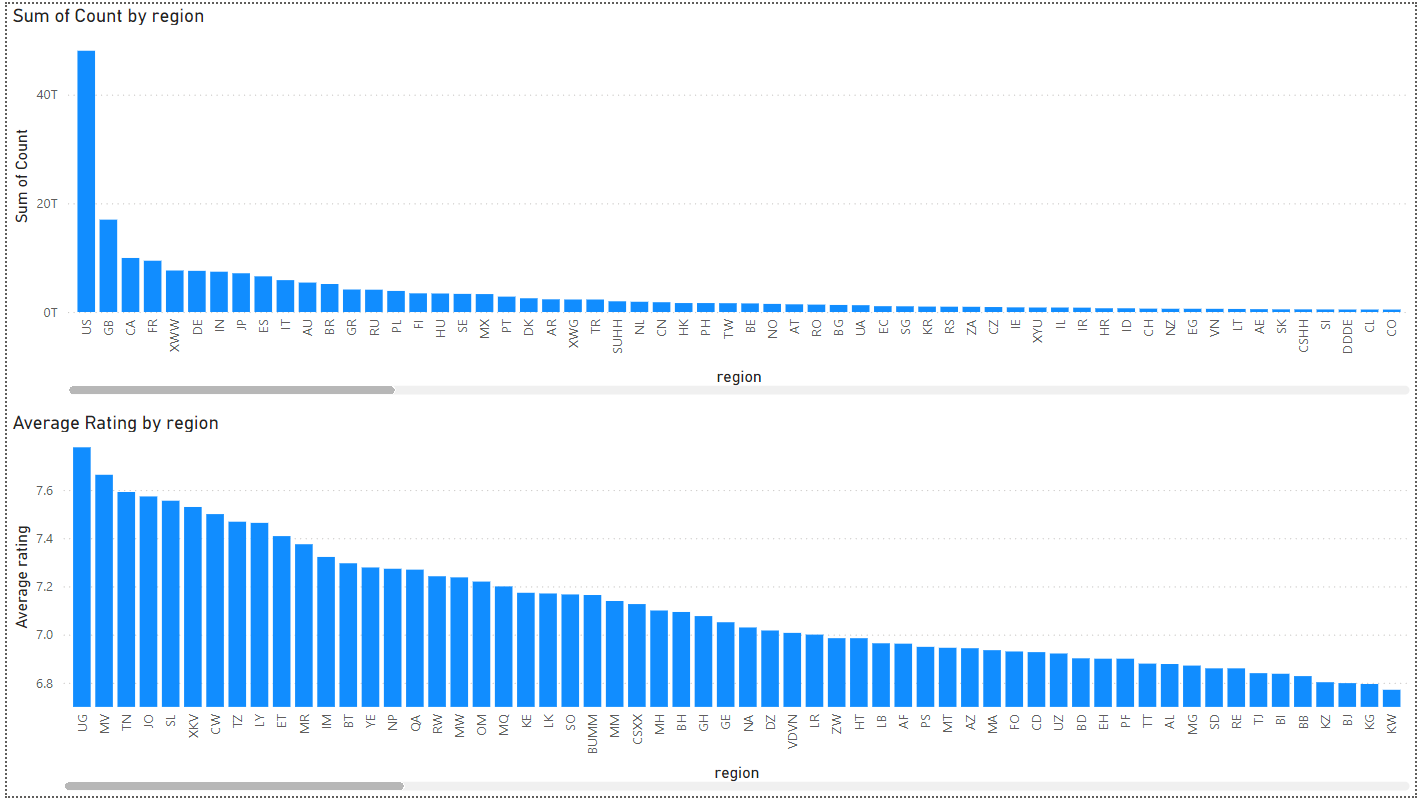
\includegraphics[width=0.8\textwidth]{../assets/movies_region.png}
    \caption{Region-wise Distribution of Movies}
    \label{fig:movies_region}
\end{figure}

% References Section
\bibliographystyle{ieeetr} % You can change to "apa" or others if required
\bibliography{references} % Create a references.bib file for bibliography entries

\end{document}
